\documentclass{article}
\usepackage{tikz}
\usetikzlibrary{arrows.meta,shapes,snakes,arrows,positioning}

\title {CP476 Final Project Proposal}
\author {Chongju Mai 150823820 \\ Zhengwen Yuan 161484420}

\tikzset{%
 	>={Latex}, 
	terminal/.style={ellipse, draw=black},
	decition/.style={diamond, draw=black,scale=0.8},
	process/.style={rectangle, rounded corners,draw=black},
	database/.style={cylinder, cylinder uses custom fill, cylinder, cylinder , shape border rotate=90, aspect=0.25, draw
    }
}

\begin{document}

\maketitle
\tableofcontents
\newpage

\section {Project Description}
This project is design to help teachers to manage their teaching materials and knowledge base. Teacher can share the file online and student can login and check look at the metrial. Student can also add comment and ask question to the teacher or other students.\\
The main demographics of this web application is teacher and students. Users does not require any special abilities to use the web application. 

\section {Requirement}

\subparagraph{} SQL Database (User info) [MySQL DB]
\subparagraph{} Storage Server (Saving files)


\section {Components}
\paragraph {Role} There are three different role in this system. Admin, Teacher, Student. Different role have different ability. Admin have the most ability and then teacher then student. i.e. Role Student can only and download teacher's file but not edit. Role will be assign when the account create.

\paragraph {User} There will be a login page and sign in page for user to sign in or sign up. Both page will communicate with user database to verify user's info. A User page will display all the info about the current user, include but not limit to username, change password, change contact info, delete account... . 

\paragraph {File System} This is the component where all the file saved. Teacher will upload the file to here so that student can view it. Due to the space limitation, each teacher can only upload certent amount of files.

\section {Milestone}

\paragraph{Backend Database} TBD 

\subparagraph{Create Database} Create the database on somehwere, maybe hopper?
\subparagraph{Create All the nessary table} After the database location is design, will manully create all the nessary table for the database. i.e. user info, files...

\paragraph{Server-side Script} TBD

\subparagraph{Account Verify} PHP script where get the form data from clinet and verify the account info 
\subparagraph{Retrive data from server} PHP script where get user data, files from the server
\subparagraph{Recive data from client and save it localy} PHP

\paragraph{Client-side Script} TBD, Will start but need to decide where is the backend server locate first. All the following will use PHP/JavaScript to implement 

\subparagraph{Send the Login/ Signup information to the Server}
\subparagraph{Upload file to the server}

\paragraph{Front End} Week 7 \\
All the following page are using the combination of HTML/CSS/JavaScript
\subparagraph{Index Page} The main page of the web application
\subparagraph{User Info Page} Page where user can manage their account
\subparagraph{Login/ Signup Page} Page where user can login /sign up
\subparagraph{Note Page} This page allow student to have their own note and todo list 
\subparagraph{Upload file/ View file page} This page is for the teacher to upload and student to view the files 

\newpage
\section{Flow Chart}
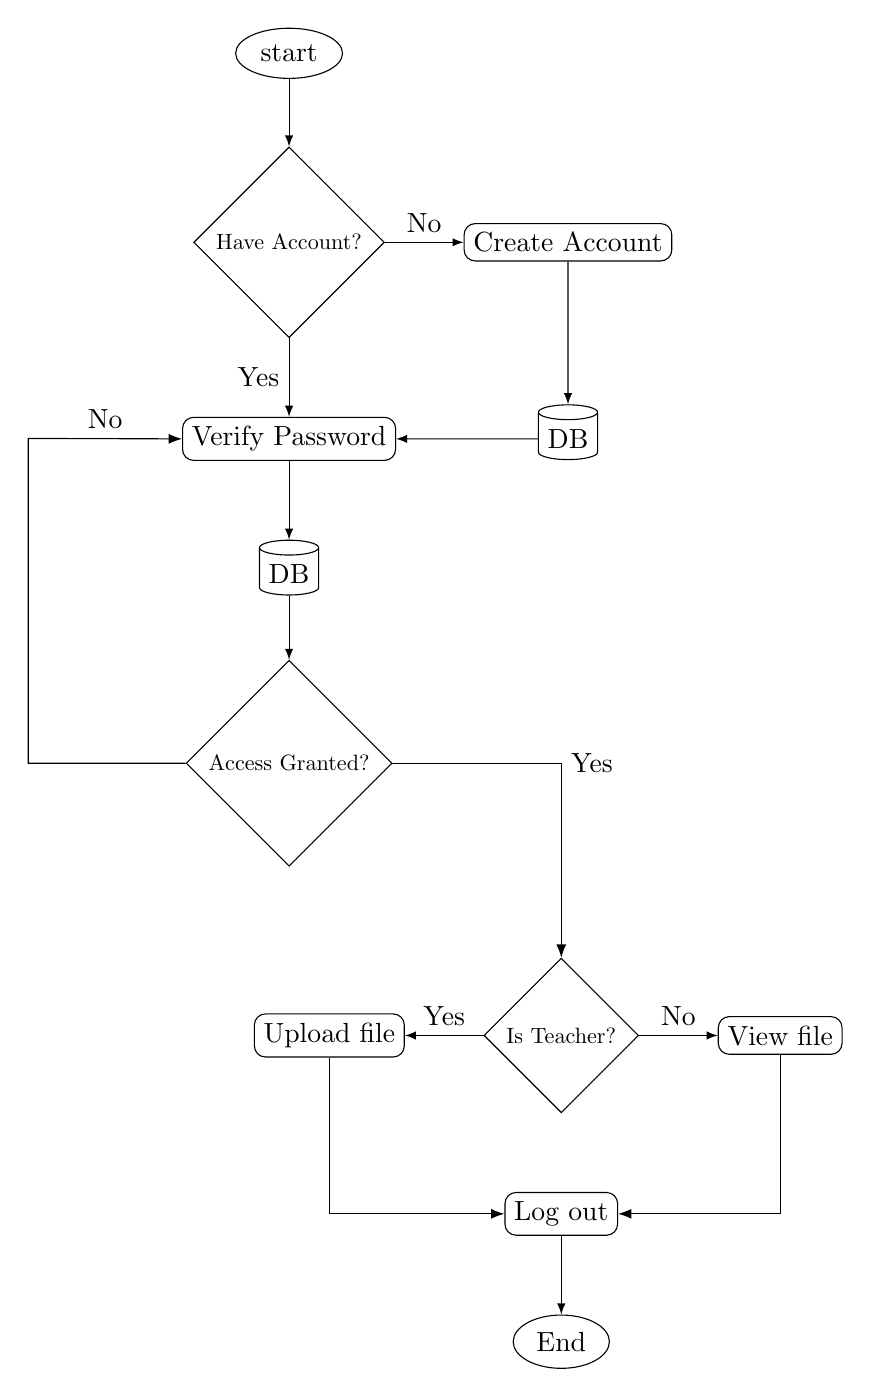
\begin{tikzpicture}[-latex,node distance=1cm, align=center,auto]
\node (start)	[terminal] {start};
\node (have_account) [decition, below of= start, yshift=-2cm] {Have Account?};
\node (r_account) [process, right= of have_account] {Create Account};
\node (p_usernamep) [process, below= of have_account] {Verify Password};
\node (d_db1) [database, right =of p_usernamep, xshift=0.8cm] {DB};
\node (d_db2) [database, below=of p_usernamep] {DB};
\node (is_correct) [decition, below of= d_db2, yshift=-2cm] {Access Granted?};
\node (is_teacher) [decition, below right =of is_correct, xshift=2cm,yshift=-2cm] {Is Teacher?};
\node (upload_file) [process, left =of is_teacher] {Upload file};
\node (view_file) [process, right =of is_teacher] {View file};
\node (logout) [process, below =of is_teacher] {Log out};
\node (end) [terminal, below =of logout] {End};

\path (start) edge (have_account);
\path (have_account) edge node[left] {Yes} (p_usernamep);
\path (have_account) edge node[above] {No} (r_account);
\path (r_account) edge (d_db1);
\path (d_db1) edge (p_usernamep);
\path (p_usernamep) edge (d_db2);
\path (d_db2) edge (is_correct);
\draw[->] (is_correct) -| node[right] {Yes} (is_teacher);
\draw[->] (is_correct.west) -- ++(-2,0) -- ++(0,2) -- ++(0,2.125) -- node[above] {No} (p_usernamep.west);
\path (is_teacher) edge node[above] {Yes} (upload_file);
\path (is_teacher) edge node[above] {No} (view_file);
\draw[->] (upload_file) |- (logout);
\draw[->] (view_file) |- (logout);
\path (logout) edge (end);

\end{tikzpicture}



\end{document}